% Appendix A
% For referencing this appendix elsewhere, use \ref{AppendixA}
\chapter{Methods} % Main appendix title
\label{Appendix-methods} 

\section{Hardware}

To run the simulation locally, a DELL Precision Tower 5810 was used, running Ubuntu 18.04, with 32GB RAM and the NVIDIA GPX 1080 graphics card with 8GB memory.

\section{AirSim}

This section describes installing AirSim on Ubuntu 20.04.

\section{CARLA Simulator Setup}

We used the CARLA fork to build UE4 (Unreal Engine 4). We followed the steps detailed in:

\begin{verbatim}
https://carla.readthedocs.io/en/0.9.12/build_linux/
\end{verbatim}

These include gathering software requirements, bulding UE4 from the CARLA UE4 fork, setting up environment variables and building CARLA.

\subsection{Running CARLA}

The top level directory level refer to is found by cloning the repository hosted at:
\begin{verbatim}
https://github.com/carla-simulator/carla
\end{verbatim}


Change directory into the repository top level, then start the simulator by running:
\begin{verbatim}
$ make launch-only
\end{verbatim}
This command launches the latest compile. To recompile before launching, run
\begin{verbatim}
$ make launch
\end{verbatim}

Once the simulator is running, the default map is loaded. This is Town10 at the time of writing. To load other maps, in the Content Browser, select folder \textbf{Carla} then \textbf{Maps} to view all maps available. If a different map is desired, double-click the map (named using the convention TownXX). The required meshes will be built if loading a town for the first time  press the play button to start. 

\begin{figure}[h!]
\centering
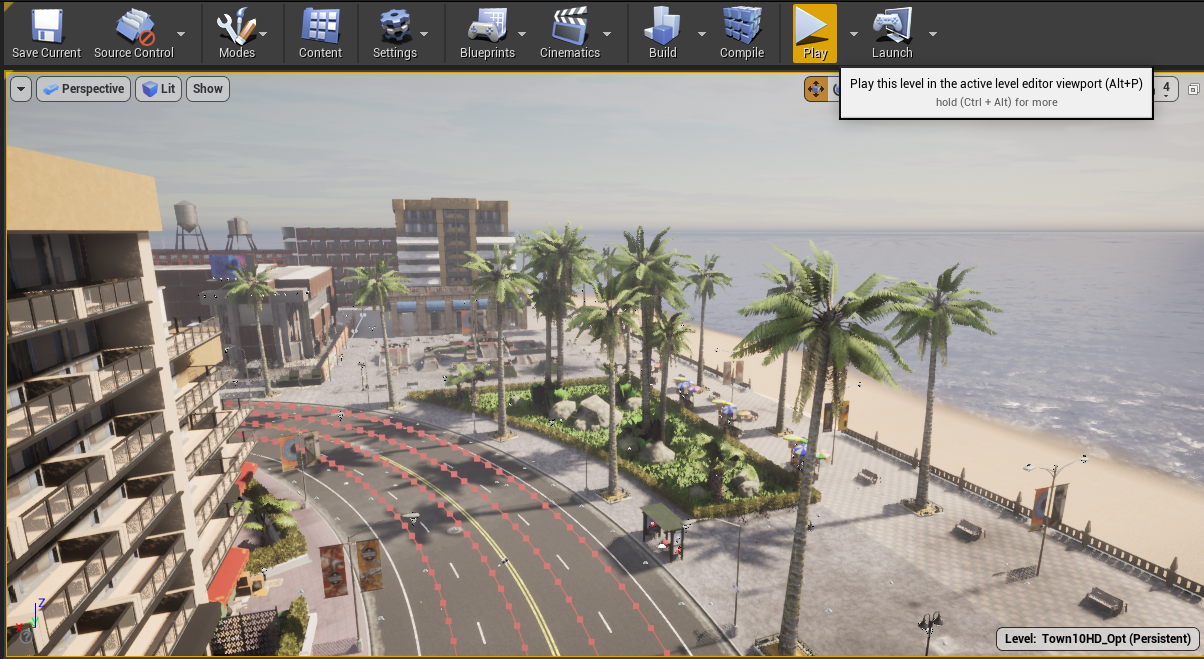
\includegraphics[width=\textwidth]{Figures/carla-play.png}
\caption{CARLA simulator running}
\label{fig:carla-play}
\end{figure}

Open a second terminal, navigate to directory:
\begin{verbatim}
carla/PythonApi/examples
\end{verbatim}
and run
\begin{verbatim}
$ python generate_traffic.py
\end{verbatim}
This will instantiate 30 vehicles and 40 pedestrians in the simulation. In a separate terminal, run
\begin{verbatim}
$ python automatic_control.py
\end{verbatim}
This will open a pygame window with one self-driving car. The screen will close once the car reaches the destination.

\section{Baidu Apollo}

Installing Baidu Apollo:
\begin{verbatim}
# clone repo
$ git clone git@github.com:ApolloAuto/apollo.git
# add env var
$ echo "export APOLLO_ROOT_DIR=$(pwd)" >> ~/.bashrc  && source ~/.bashrc
# install docker and add write rights to socks
$ sudo snap install docker
$ sudo chmod 666 /var/run/docker.sock
# change directory and download docker image
# cd apollo
$ bash docker/scripts/dev_start.sh 
\end{verbatim}

\subsection{HPC - Hyperion Cluster}
To access the cluster, we open a VPN tunnel with PulseUI or similar:
% TODO write up properly
%1. Connect to PulseUI
%2. On one shell:
%ssh -N  aczd097@10.200.51.10 -L 2002:hyperion.city.ac.uk:22
%3. On the other:
%ssh -p2002 aczd097@localhost

%where the port number may be any value from 2000 to 3000 inclusive and must match in steps 3, 4 and 6.

%# Activate gridware

%flight env activate gridware

%# list modules

%module avail

%# load module

%module load apps/python3

% From Angelina Nazev
HPC Introduction Session 1 (28/9)

https://web.microsoftstream.com/video/e1cfc0bb-9e74-4677-b40b-4e26870e5eb8

 

HPC Introduction Session 2 (29/9)
https://web.microsoftstream.com/video/8ad789f3-4b3d-4e4e-8e8d-f5be80b06057

 

HPC Introduction Session 3 (18/10)

https://web.microsoftstream.com/video/f9c4bddc-2185-497c-8626-3351b562ef9c

HPC Introduction Session 4 (20/10)

https://web.microsoftstream.com/video/669b50de-f870-4294-8a0c-04eea196765e

HPC More info:
https://www.city.ac.uk/about/facilities/specialist-facilities/high-performance-computing

HPC Guidance pages:
%https://cityuni.service-now.com/sp?id=search&spa=1&q=HPC
